\section{Introduction and main results}

\begin{frame}{Introduction}
  \begin{spaceditemize}
    \item Learning (properties of) quantum states as efficiently as possible is a fundamental task in quantum information
    \item There is a lot of recent work on learning continuous variable (CV) states (eg.~\cite{mele2024learning-quantu,zhao2024complexity-of-q,bittel2025energy-independ,fanizza2025efficient-learn})
    \item Most \emph{sample and time efficient} learning algorithms work for \textbf{Gaussian} or \textbf{near-Gaussian} states
    \item Learning a generic \( n \)-mode CV state requires \( \sim (\text{energy})^n \) samples \parencite{mele2024learning-quantu}
  \end{spaceditemize}
\end{frame}

\begin{frame}{Our goal}
  \begin{minipage}{.49\textwidth}
    \begin{spaceditemize}
      \item Our goal is to find interesting, \textbf{highly non-Gaussian} classes of CV states with \emph{sample and time efficient} learning algorithms
      \item Motivated by an open problem proposed in \cite{aaronson2023efficient-tomog}, we start with \textbf{BosonSampling states}
    \end{spaceditemize}
  \end{minipage}
  \hfill
  \begin{minipage}{.49\textwidth}
    \begin{center}
      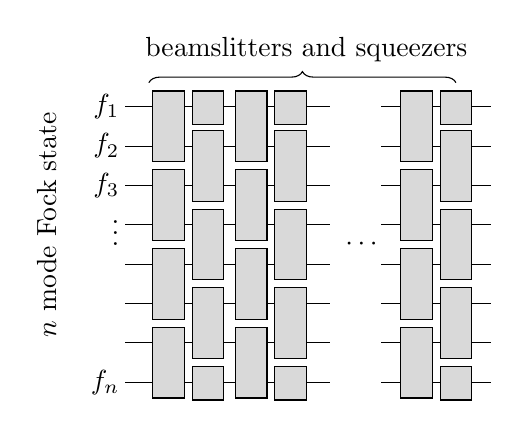
\begin{tikzpicture}
        \foreach \mode in {1,...,8}{
            \draw (.5,-\mode/2) --++ (2.6,0);
            \draw (3.75,-\mode/2) --++(1.4,0);
            \ifnum\mode < 4
              \node[left] at (.55,-\mode/2) {\(\ket{f_{\mode}}\)};
            \fi
          }
        \node[left] at (.55,-4) {\(\ket{f_n}\)};
        \node[left] at (.55,-2) {\(\vdots\)};
        \begin{scope}[yshift=-.3cm,xshift=-.2cm]
          \foreach \layer in {1,2,4}{
              \begin{scope}[xshift=\layer*.05cm]
                \foreach \lbrick in {0,...,3}{ % make left layer U(2) blocks
                    \draw[fill=gray!30] (\layer,-\lbrick) rectangle (\layer+.4,-\lbrick-.9);
                  }
                \foreach \rbrick in {0,...,2}{ % make right layer U(2) blocks
                    \draw[fill=gray!30,yshift=-.5cm,xshift=.5cm] (\layer,-\rbrick) rectangle (\layer+.4,-\rbrick-.9);
                  }
                % R layer top and bottom U(1) blocks
                \draw[fill=gray!30,xshift=.5cm] (\layer,0) rectangle (\layer+.4,-.425);
                \draw[fill=gray!30,xshift=.5cm] (\layer,-3.5) rectangle (\layer+.4,-3.5-.425);
              \end{scope}
            }
          \draw[decoration={brace,raise=3pt,aspect=.5,amplitude=4pt},decorate] (1,0)--(4.9,0);
          \node[above] at (3,0.25) {beamslitters and squeezers};
        \end{scope}
        \node at (3.5,-2.25) {\(\cdots\)};
        \node[rotate=90] at (-.5,-2) {\(n\) mode Fock state};
      \end{tikzpicture}
    \end{center}
  \end{minipage}
\end{frame}


%%%%%%%%%%%%%%%%%

\begin{frame}{Background}

  \begin{spaceditemize}
    \item A bosonic system of \(n\) modes is described by the creation and annihilation operators \(a_1^\dag,\dots,a_n^\dag, a_1, \dots, a_n\)
    \item Equivalently, by position and momentum operators \(\bm r = (x_1, \dots, x_n, p_1, \dots, p_n)\)
    % \item These obey the CCR $[r_i, r_j] = \i \Omega_{ij}$, with
    % \[\Omega = \begin{pmatrix}
    %     0 & \bbI \\ - \bbI & 0
    %   \end{pmatrix}\]
    % \item A unitary transformation must perserve the CCR
    % \[[\calU r_i\calU^\dag, \calU r_j\calU^\dag] = \calU [r_i, r_j] \calU^\dag = \i\calU \Omega_{ij} \calU^\dag = \i\Omega_{ij}\]
    \item A unitary transformation is called \textit{Gaussian} if it acts affinely on \(\bm r\)
    \[\calU_{S, \bm d}^\dag r_i \calU_{S, \bm d} = d_i + \sum_{j} S_{ij}r_j \]
    % \item To preserve the CCR, $S$ must satisfy $S \Omega S^T = \Omega$
    % \[S \in \Sp(2n, \bbR) \coloneqq \set{S \in \GL(2n, \bbR) \mid S \Omega S^T = \Omega}\]
    % \item Easy to see the composition $\calU_{S, \bm d} \calU_{R, \bm e} = \calU_{SR, R \bm d + \bm e}$
    \item \textbf{The group of Gaussian unitaries is} \(\Sp(2n, \bbR)  \ltimes \bbR^{2n}\)
  \end{spaceditemize}

\end{frame}


%%%%%%%%%%%%%%%%%


\begin{frame}{Problem statement \parencite{aaronson2023efficient-tomog}}
  \begin{minipage}{.7\textwidth}
    \begin{spaceditemize}
      \item Let \(\ket{\bm f}\) denote an unknown Fock state on \(n\) modes, \(\bm f = (f_1,\dots, f_n) \in \bbN_0^n\)
      \item Let \(\calU_S\) denote a Gaussian unitary specified by an unknown matrix \(S \in \Sp(2n, \bbR)\)
      \item Let \(\ket{\psi} = \calU_S \ket{\bm f}\) \pause
      \item Given \(N\) copies of \(\psi\), we want to learn \(\psi\) to \(\varepsilon\) precision
      \item Find a \(\bm g\) and \(Q\) such that \(\abs*{\bra{\bm g}\calU_Q^\dag \calU_S \ket{\bm f}} \geq 1 - \varepsilon\)
    \end{spaceditemize}
  \end{minipage}
  \hfill
  \begin{minipage}{.29\textwidth}
    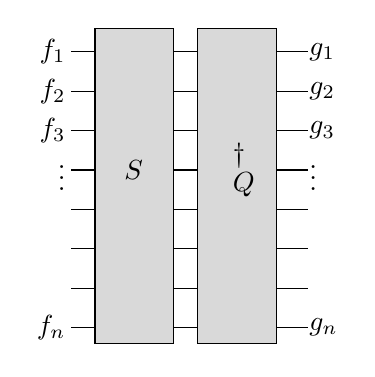
\begin{tikzpicture}
      \foreach \mode in {1,...,8}{
          \draw (.5,-\mode/2) --++ (3,0);
          \ifnum\mode < 4
            \node[left] at (.55,-\mode/2) {\(\ket{f_{\mode}}\)};
            \node[right] at (3.4,-\mode/2) {\(\ket{g_{\mode}}\)};
          \fi
        }
      \node[left] at (.55,-4) {\(\ket{f_n}\)};
      \node[left] at (.55,-2) {\(\vdots\)};
      \node[right] at (3.4,-4) {\(\ket{g_n}\)};
      \node[right] at (3.4,-2) {\(\vdots\)};
      \draw[fill=gray!30] (.8,-0.2) rectangle (1.8,-4.2);
      \node at (1.3,-2) {\Large \(\calU_S\)};
      \draw[fill=gray!30] (2.1,-0.2) rectangle (3.1,-4.2);
      \node at (2.7,-2) {\Large \(\calU_Q^\dag\)};
    \end{tikzpicture}
  \end{minipage}
  \pause
  \vfill
  \begin{block}{}
    \begin{itemize}
      \item How large must \(N\) be? ~~~~~~~~~~~~~~~~~~~~~~~~~~\textit{Want it to be \(\leq \poly{\rm energy}\)}
      \item What is the measurement scheme?~~~~~~~~~~~~\textit{Want it to be practically accessible}
      \item How hard is the classical postprocessing?~~~~\textit{Want it to be \(\leq \poly{n}\)}
    \end{itemize}
  \end{block}
\end{frame}


\begin{frame}{Analogous fermionic problem}
  \begin{spaceditemize}[2em]
    \item The analogous fermionic problem was solved in \cite{aaronson2023efficient-tomog}
    \item Crucial difference: fermionic Fock states are Gaussian, bosonic Fock states are highly non-Gaussian
  \end{spaceditemize}
\end{frame}





\begin{frame}{First main result}
  \begin{spaceditemize}
    \item We will solve this problem with \textit{moments} for \( \ket\psi = \calU_S\ket{\bm f}\)
    \begin{equation*}
      \Lambda^{(t)}_{i_1,\dots,i_t; j_1,\dots,j_t} = \bra\psi r_{i_1}\dots r_{i_t} r_{j_1}\dots r_{j_t}\ket\psi
    \end{equation*}
    \item Suppose we know \(\Lambda^{(1)\prime},\Lambda^{(2)\prime}\) such that \(\norm*{\Lambda^{(t)\prime} - \Lambda^{(t)}} \leq \varepsilon_t\)
    \pause
  \end{spaceditemize}

  \begin{theorem}
    We find an \textbf{efficient} algorithm that finds a \(Q\) and \(\bm g\) such that
    \begin{equation*}
      \abs*{\bra{\bm f}\calU_S^\dag \calU_Q \ket{\bm g}} \geq 1 - \bigO{\varepsilon_1 n^2 \norm*{\bm f}_\infty^3 \norm*{S^TS}^{3/2} + \varepsilon_2 n^2 \norm*{\bm f}_\infty \norm*{S^TS}^3}
    \end{equation*}
  \end{theorem}

  This can therefore be combined with \textit{any} strategy to measure moments to yield a \textbf{sample and time efficient learning algorithm}
\end{frame}


\begin{frame}{Measuring moments}

  \begin{theorem}
    Using a \textbf{median of means} estimator,
    \(\Lambda^{(2t)}\) for \(\calU_S\ket{\bm f}\) can be estimated to norm precision \(\varepsilon\) with probability at least \(1-\delta\) using
    \(N \sim \bigO{\frac{\log(n/\delta)}{\varepsilon^2} \parentheses{n\norm*{f}_\infty \norm*{S^TS}}^{2t}}\) \textbf{heterodyne} samples.
  \end{theorem}

  \pause

  \vfill

  \begin{corollary}[Full solution to \cite{aaronson2023efficient-tomog}]
    \(N\) heterodyne samples from the state \(\calU_S\ket{\bm f}\) suffice via our efficient algorithm to learn a \(Q,\bm g\) satisfying \(\abs*{\bra{\bm f}\calU_S^\dag \calU_Q \ket{\bm g}} \geq 1 - \gamma\) with probability at least \(1-\delta\), where
    \begin{equation*}
      N \sim \bigO{\frac{\log(n/\delta)}{\gamma^2} n^8 \norm*{\bm f}_\infty^{10} \norm*{S^TS}^{10}}
    \end{equation*}
  \end{corollary}

  \vfill

  Roughly, \(n \norm{\bm f}_\infty \norm*{S^TS} \sim \) energy


\end{frame}






%%%%%%%%%%%%%%%%%
\section{Sample efficiency}
\overviewslide[currentsection]


\begin{frame}{\Gt states}
  \begin{definition}
    A \Gt state is a thermal (or ground) state of a (non-degenerate) Hamiltonian that is degree \(t\) in the quadrature operators
  \end{definition}

  \vfill

  \begin{spaceditemize}
    \item A \Gt state is \textbf{fully specified} by its first \(t\) moments
  \end{spaceditemize}
\end{frame}


\begin{frame}{Pure \Gt states}

  \begin{spaceditemize}
    \item Suppose \(\psi\) is a \Gt state; it is the ground state of \(H = \sum_i \alpha_i \hat M_i\) where \(\hat M_i\) are degree \(\leq t\) operators
    \pause
    \begin{align*}
      \bra\psi H \ket\psi
      %
       & = \min_\phi \sum_i \alpha_i \bra\phi \hat M_i \ket\phi                                                     \\
      %
       & = \min_{m_1,m_2,\dots} \sum_i \alpha_i m_i \quad \text{st } \exists \phi, \bra\phi \hat M_i \ket\phi = m_i
    \end{align*}
    \pause
    \item Because \(H\) is non-degenerate, any state with the matching moments is \(\psi\) \pause
    \item If \(H\) is \emph{gapped}, then \textbf{inverse poly moment precision corresponds to inverse poly state fidelity} \parencite{yu2023learningmarginalssuffices}
  \end{spaceditemize}

\end{frame}


\begin{frame}{Relevance to the learning algorithm}
  \begin{spaceditemize}
    \item A Fock state \(\ket{\bm f}\) is a \G4 state; it is the ground state of
    \(H = \sum_i (\hat a_i^\dag \hat a_i - f_i)^2\)
    \item The set of \Gt states is closed under the action of Gaussian unitaries (because they act affinely)
    \pause
    \item Therefore, \(\calU_S\ket{\bm f}\) is the ground state of a gapped degree \(4\) Hamiltonian
    \item Knowing the \textbf{first four moments to inverse poly precision} suffices to learn the state
    \pause
    \item But this does \emph{not} guarantee a time-efficient learning algorithm
  \end{spaceditemize}
\end{frame}


%%%%%%%%%%%%%%
\section{Time efficiency}
\overviewslide[currentsection]


\begin{frame}{Sketch of our algorithm}
  \begin{spaceditemize}
    \item For simplicity, we will restrict our attention here to \\[1em]
    ~~~~~passive Gaussian unitaries (specified by \(W \in \U(n)\))\\[1em]
    ~~~~~the Fock state \(\ket{1,\dots,1} \equiv \ket{1^n}\)\\[1em]
    ~~~~~the error free case (assume moments are known \emph{perfectly})\\[1em]
    \pause
    \item We sketch the learning algorithm with these simplicifcations
  \end{spaceditemize}

\end{frame}

\begin{frame}{Passive moment transformations}
  \begin{spaceditemize}
    \item Recall \( W\in U(n) \) acts as
    \[\calU_W^\dag a_i \calU_W = \sum_{j} W_{ij} a_j \]
    \item How do moments \textbf{transform}?
    \begin{align*}
       & \sigma^{(t)}_{i_1,\dots,i_t; j_1,\dots,j_t} = \bra{1^n}\calU_W^\dag a_{i_1}\dots a_{i_t}a^\dag_{j_1}\dots a^\dag_{j_t} \calU_W\ket{1^n} \\
      %
       & (\sigma^{(t)}_0)_{i_1,\dots,i_t; j_1,\dots,j_t} = \bra{1^n} a_{i_1}\dots a_{i_t}a^\dag_{j_1}\dots a^\dag_{j_t}\ket{1^n}                 \\
      %
       & \sigma^{(t)} = W^{\otimes t}\sigma^{(t)}_0 W^{\dag \otimes t}
    \end{align*}
    %
    \item \(\sigma^{(t)}\) is a submatrix of a unitary transformation of the \(\Lambda^{(t)}\) moments
  \end{spaceditemize}

\end{frame}


\begin{frame}{Reducing the problem}
  \begin{spaceditemize}
    \item If we were dealing with Gaussian states, \(\sigma^{(1)}\) would be sufficient
    \pause
    \item But for us \textbf{second moments are useless} --- easy to check that \(\sigma^{(1)}_0 \propto \bbI\)
    \item Therefore, \(\sigma^{(1)} = W \sigma^{(1)}_0 W^\dag = \sigma^{(1)}_0\), so we learn nothing about \(W\) by measuring second moments
    \pause
    \item So now we use \textbf{fourth moments}, \(\sigma^{(2)}\)
  \end{spaceditemize}
\end{frame}


\begin{frame}{Learning algorithm}
  \begin{block}{}
    Given the fourth moments \(\sigma^{(2)} = W^{\otimes 2} \sigma^{(2)}_0 W^{\dag \otimes 2}\) for the state \(\calU_W \ket{1^n}\), determine \(W\)
  \end{block}
  \vfill
  \pause
  \begin{spaceditemize}[0em]
    % \item Recall we are still assuming that $\sigma^{(4)}$ is known perfectly
    \item Because \( \sigma^{(2)}_0 \) is a matrix on \( (\bbC^{n})^{\otimes 2} \), we can represent it in bra-ket notation using the standard basis \( \ket{1},\dots,\ket{n} \) of \( \bbC^n \)
    % .
    % Easy to check that 
    \begin{equation*}
      \sigma^{(2)}_0 = 4 (\bbI + U_{\rm SWAP})
      - 2\sum_{i=1}^{n}\ket{i,i}\bra{i,i},
    \end{equation*}
    \pause
    \item Denote the \( i^{\rm th} \) column vector of \( W \) by \( \ket{w_i} \).
    Given access to \(\sigma^{(2)}\), we can thus form the matrix
    \begin{align*}
      A & = \frac{1}{2}\parentheses{4(\mathbb I + U_{\rm SWAP}) - \sigma^{(2)}}     \\
      %
        & =  \sum_{i=1}^n (\ket{w_i}\otimes \ket{w_i})(\bra{w_i}\otimes \bra{w_i}),
    \end{align*}
  \end{spaceditemize}
\end{frame}

\begin{frame}{Learning algorithm}
  \begin{block}{}
    Given access to a matrix \(A = \sum_{i=1}^n (\ket{w_i}\otimes \ket{w_i})(\bra{w_i}\otimes \bra{w_i})\), learn \(\ket{w_i}\) (up to phases and permutations)
  \end{block}
  \vfill
  \pause
  \begin{spaceditemize}
    \item Unitarily diagonalize \(A\) and take the \(+1\) eigenvalues --- we learn the eigenspace \(\text{span}\cbargs{\ket{w_i}\otimes \ket{w_i} \mid i=1,\dots, n}\)
    \pause
    \item A numerical diagonalization routine will return the vectors
    \begin{equation*}
      \ket{\tilde w_i} = \sum_{j=1}^n U_{ij}\ket{w_j}\otimes \ket{w_j}
      =
      \sum_{j=1}^n \abs*{U_{ij}}e^{\i\phi_{ij}}\ket{w_j}\otimes \ket{w_j}
    \end{equation*}
    \item The unitary \(U\) is totally arbitrary and unpredictable
  \end{spaceditemize}
\end{frame}


\begin{frame}{Learning algorithm}
  \begin{block}{}
    Given access to the vectors \(\ket{\tilde w_i} = \sum_{j=1}^n \abs*{U_{ij}}e^{\i\phi_{ij}}\ket{w_j}\otimes \ket{w_j}\) with \(U,\phi\) unknown and arbitrary, learn \(\ket{w_j}\) (up to phases and permutations)
  \end{block}
  \vfill
  \pause
  \begin{spaceditemize}
    \item Take the intersection of the Schmidt decompositions of all \(\ket{\tilde w_i}\) to learn all the \(\ket{w_i}\) up to phases
    \pause
    \item We define \( V \) to be the unitary matrix whose columns are precisely these learned vectors
    \item By construction, \( V \) is equal to \( W \) up to a permutation of its columns and global phases applied to the columns
  \end{spaceditemize}

\end{frame}

\begin{frame}{Learning algorithm}

  \begin{spaceditemize}[2em]
    \item In other words, we have learned the matrix \(V = W \Phi P\), where \(\Phi\) is some arbitrary diagonal unitary matrix, and \(P\) is some arbitrary permutation matrix
    \item It follows that the state \( \calU_V \ket{1^n} \) is the same as \( \calU_W \ket{1^n} \) up to an irrelevant global phase, thereby completing the learning algorithm
    \pause
    \item To prove the main result, we need to track how the error in the moments propagates through the algorithm to an error in the fidelity
  \end{spaceditemize}

\end{frame}


%%%%%%%%%%%%%%%%%
\section{Outlook}
\overviewslide[currentsection]


\begin{frame}{Summary}
  \begin{spaceditemize}
    \item By going beyond second moments, we found a \textbf{sample and time efficient} algorithm to learn \emph{BosonSampling states}
    \item Solves open problem left by \cite{aaronson2023efficient-tomog}
    \pause
    \item We construct an \textbf{infinite set of Gaussian invariants for generic bosonic states} using classical invariant theory of the action of symplectic group on moments, relevant for state conversion \parencite{chabaud2020stellar-represe,hahn2024assessing-non-g}
    \pause
    \item Lots of possible extensions!
  \end{spaceditemize}
\end{frame}

\begin{frame}{Extensions}
  \begin{spaceditemize}
    \item Our algorithm generalizes to a slightly larger class of states, and fails interestingly in other places
    \item Certain classes of states \emph{hide information} from lower moments
    \item Invariants and generalizations of Wick's theorem
    \pause
    \item Can we make our algorithm have more favorable scaling with energy? \\[1em]
    \hspace{1em} \textbullet ~ Our algorithm requires \textcolor{red}{\(N \sim \poly*{n, \norm*{\bm f}_\infty, \norm*{S^TS}}\)} samples \\[1em]
    \hspace{1em} \textbullet ~ Applying \parencite{bittel2025energy-independ}, we get
    \textcolor{red}{\(N \sim \poly*{n, \norm*{\bm f}_\infty, \log \norm*{S^TS}}\)}
  \end{spaceditemize}
\end{frame}
